\documentclass[10pt]{article}\usepackage[margin=.65in]{geometry}\usepackage[T1]{fontenc}\usepackage{graphicx}\setlength{\parindent}{0pt}\setlength{\parskip}{7pt}\sloppy\begin{document}{\large Union, polynomial division and runtime prerequisites}\par This packet advances the signed-graph union invariant and the monic quotient correspondence, and independently checks the proposed mount-diff parser. A separately built native checker and independent integer recomputation also verify the retained Kummer matrix bindings. These are formal, source and saved-certificate results; the original 1,260-target scientific scope is unchanged.\par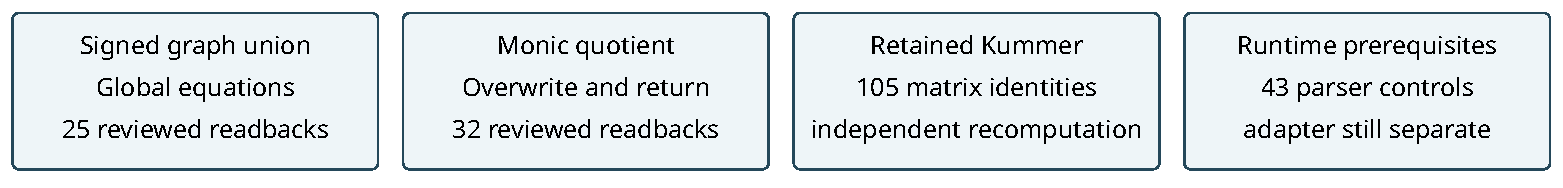
\includegraphics[width=\linewidth]{diagram.pdf}\par Union mutation. Five main declarations, eight producer controls and twelve independent reviewer controls passed twenty-five named axiom readbacks. The invariant covers every vertex equation and every stored anchor through either union direction, including signed descendants and a retained child anchor. Both-fixed roots yield the correct target when the constraint coefficient is nonzero, and consistency when it is zero. The model starts after find; forest/size preservation, allocation and concrete storage remain separate.

Monic division. Seventeen main declarations, nine producer controls and six independent reviewer controls passed thirty-two named axiom readbacks. The proof models coefficient overwrite, proves each selected quotient slot is fresh, preserves A=QB+R, and proves termination and the exact returned quotient. It uses the existing checked word-remainder loop under canonical monic inputs and prime p$<$2\textasciicircum{}31. Native quotient-vector storage/trim and general nonmonic inverse/extended-GCD behavior remain separate.

Retained Kummer matrices. All 105 ordered matrices across the 21 models satisfy M\textasciicircum{}2=cI with nonzero c and match the saved scalars. Twelve historical source pins match. Independent integer recomputation agrees on every matrix and normalized root; eight adverse controls preserve the distinction between native rejection, inventory rejection and external source-binding rejection. The checker alone accepts an altered walk file, so exact frozen hashes are a required acceptance component. Native row-fold and executed-binary provenance remain separate.

Runtime parser. Independent fixed controls accepted seven cases and rejected thirty-six malformed cases. Accepted records retain writer\_attribution=null and no\_writes\_claim=false. Historical qualification v5 remains failed with Q0 alone passed. The actual supervisor still requires empty diff; the reviewed parser is not integrated. AMENDMENT\_REQUIREMENTS.md lists the precise callsite, identity, transport, binding and qualification obligations.

Review sequence. The prospective joint plan was published before cross-review. Producer proof sources were published before independent review dispatch. All initial failures and source snapshots remain in the packet. Compiler success, named axiom inventories and source-fidelity review are separately recorded. No new scientific execution, timing measurement or cost ratio is supplied by this packet.
\end{document}